

\chapter{Overview dell'architettura e delle componenti utilizzate}

\label{ch:overview}

\section{Obbiettivo da ottenere \workinprogress}

\todo[la sezione è da espandere! in qualche modo]

In una collaborazione tra il Dipartimento di Ingegneria dell'Informazione e l'azienda \textbf{Esse-ti S.R.L.} ci è stato esposto un progetto che consiste nel:

%todo non mi piace come sta messo
\begin{itemize}
	\item Fornire a dei clienti un router 4G, su cui possono essere connessi vari dispositivi, ad es. di tipo domotico.
	\item Rendere questi dispositivi accessibili ai clienti attraverso internet
\end{itemize}

\begin{figure}[H]
	\centering
	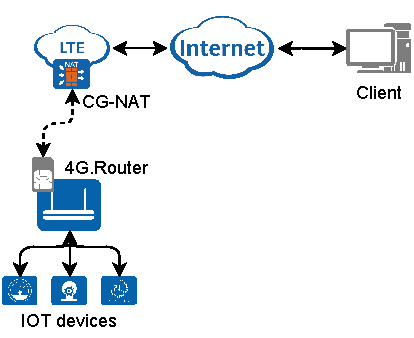
\includegraphics[width=0.5\linewidth]{immagini/diag-goal}
	\caption{Schema concettuale dell'obbiettivo da raggiungere.}

	\label{fig:schema_concettuale}

\end{figure}

Data la presenza del NAT si vede subito che non è realizzabile a meno che il cliente non abbia un'IP pubblico e la sua macchina venga configurata opportunamente. Questo però non è possibile nel caso generale, quindi per risolvere efficacemente questa topologia si deve necessariamente introdurre una terza macchina provvista di IP pubblico e che funga da ponte tra il \textit{4G.Router} e il cliente.


\begin{figure}[H]
	\centering
	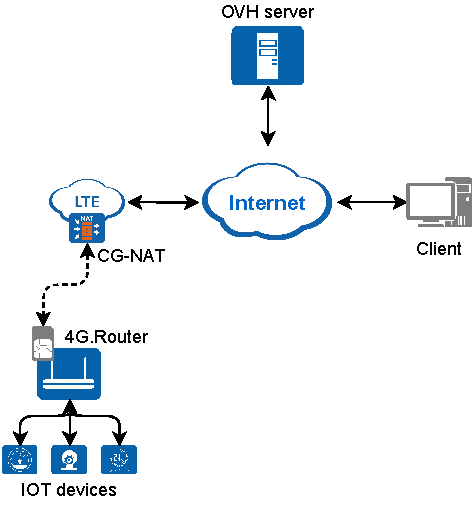
\includegraphics[width=0.5\linewidth]{immagini/diag-real}
	\caption{Schema concettuale dell'architettura che si dovrà implementare.}
	\label{fig:schem_architettura_reale}
\end{figure}

In questo modo si può usare il \textit{Server} per configurare una \textit{Virtual Private Network} (VPN), a cui saranno connessi sia il \textit{4G.Router} che il cliente. Ciò consente la creazione di una topologia virtuale in cui tutti i dispositivi connessi alla VPN sono nella stessa rete locale, quindi possono comunicare tra loro.

Inoltre in questo modo viene minimizzata la configurazione da effettuare sulle macchine dei clienti, infatti sarà sufficiente avere un client OpenVPN.

La configurazione virtuale vista dal 4G.Router e dai clienti sarà quindi:

\begin{figure}[H]
	\centering
	\includegraphics[width=0.5\linewidth]{immagini/diag-virtual}
	\caption{Topologia virtuale vista dal cliente.}
	\label{fig:schema_architettura_virtuale}
\end{figure}

\newpage
\section{Specifiche dei componenti}

% TODO da espandere in qualche modo così è veramente brutto!

Per la realizzazione di questa topologia sono necessari i seguenti componenti:

\begin{itemize}
	\item Esse-ti 4G.Router
	\item Server
	\item Host domotico
	\item Macchina del cliente
\end{itemize}

Alcuni di questi componenti necessiteranno di delle caratteristiche specifiche.

\subsection{Esse-ti 4G.Router \workinprogress}

Ci è stato fornito dall'azienda Esse-ti, consiste in un gateway 4G con funzionalità di router. Le specifiche complete possono essere trovate sul sito del produttore (\href{https://www.esse-ti.it/4g-router}{link}).


\begin{figure}[ht]
	\centering
	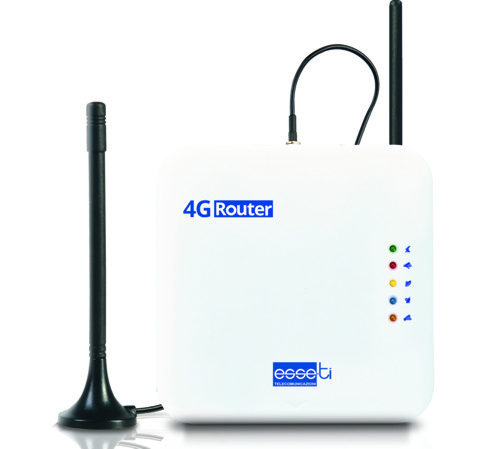
\includegraphics[width=250px]{immagini/4grouter.jpg}
	\caption{Esse-ti 4G.Router}
	\label{fig:esse-ti-router-4g}
\end{figure}

Per l'implementazione di questa architettura sono necessarie solo un sub-set delle specifiche:


\begin{itemize}
	\item Access Point wireless per offrire connettività Internet Wi-Fi
 
	\item Client Dynamic DNS per consentire all’utente di raggiungere da remoto, tramite Internet, il router stesso e tutti i dispositivi connessi via Wi-Fi o porta LAN
	
	\item Gateway telefonico per consentire l’invio e la ricezione di chiamate attraverso la rete 4G LTE/UMTS/GSM a telefoni fissi
\end{itemize}

% TODO nooop
Ha il sistema operativo \textit{Draghino}, una versione personalizzata di OpenWRT, in cui è stata modificata l'interfaccia web... mh no

La configurazione del dispositivo può essere fatta sia da terminale, entrando in ssh, sia da interfaccia web:

\begin{figure}[H]

	\newlength{\tempheight}
	\setlength{\tempheight}{23ex}

	\centering%
	\begin{subfigure}[t]{0.5\textwidth}
		\centering%
		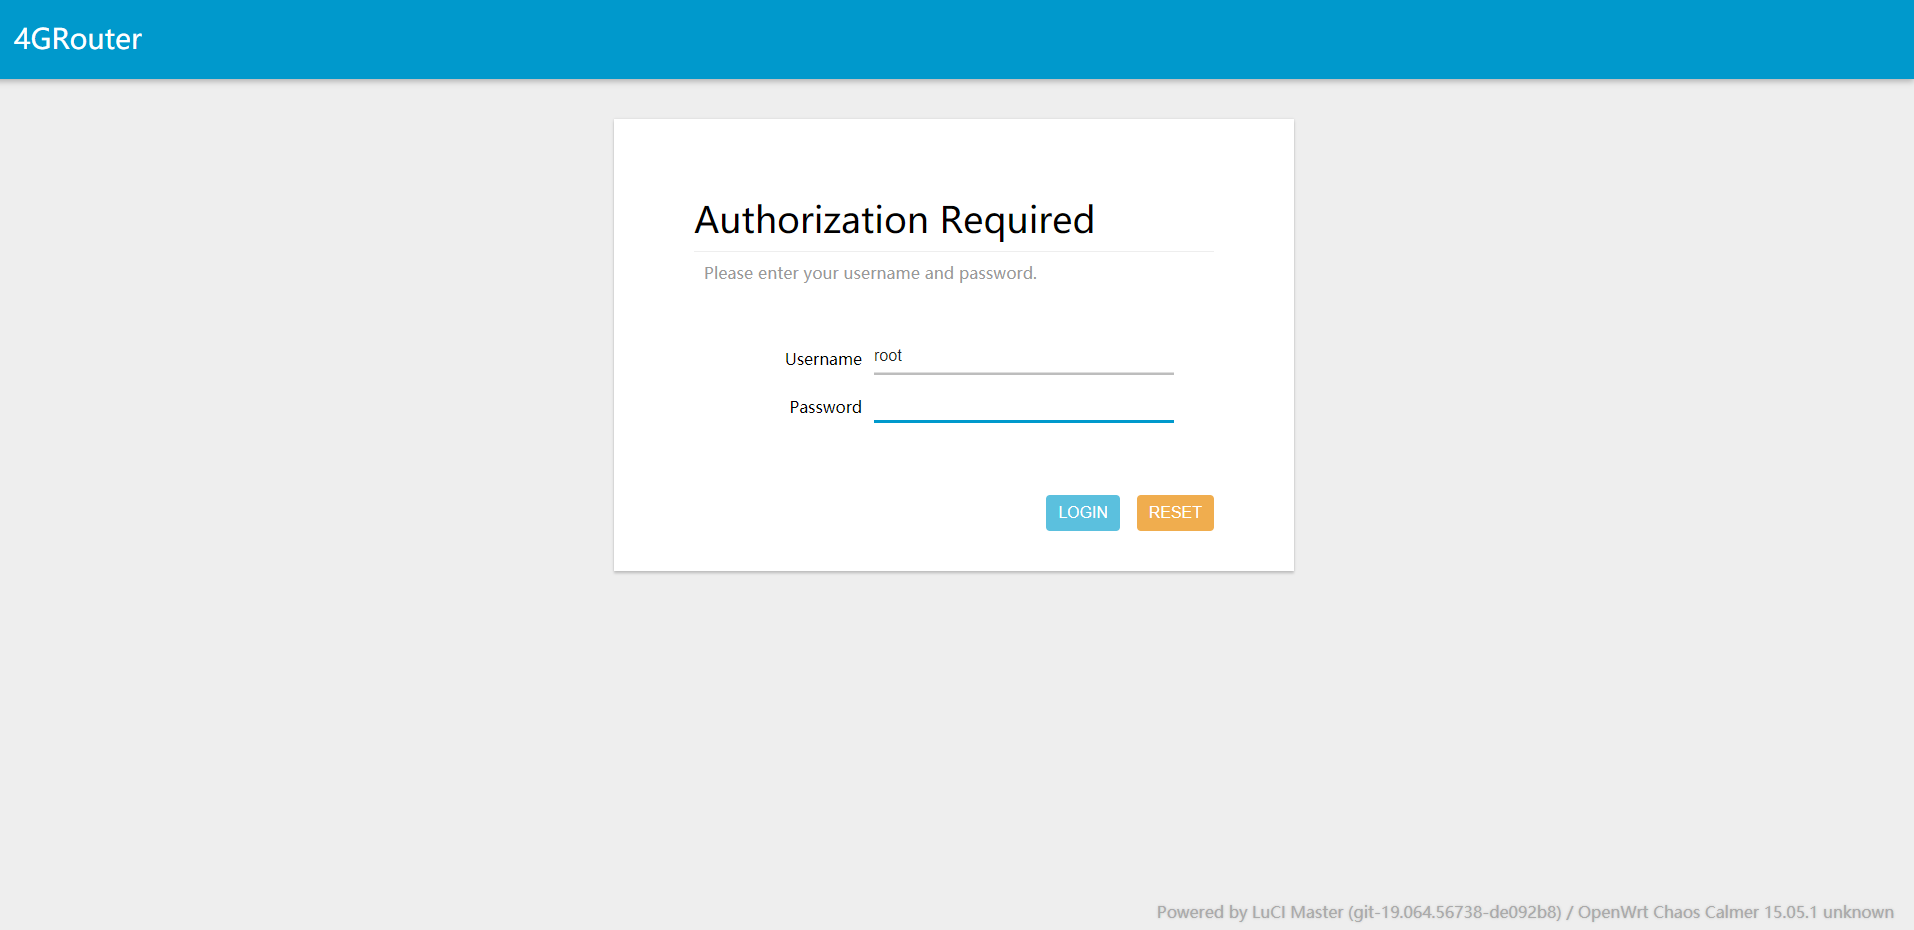
\includegraphics[totalheight=\tempheight]{immagini/interfacciar4g_init}
		\caption{Schermata di autenticazione}
	\end{subfigure}%
	\hfill
	\begin{subfigure}[t]{0.5\textwidth}
		\centering%
		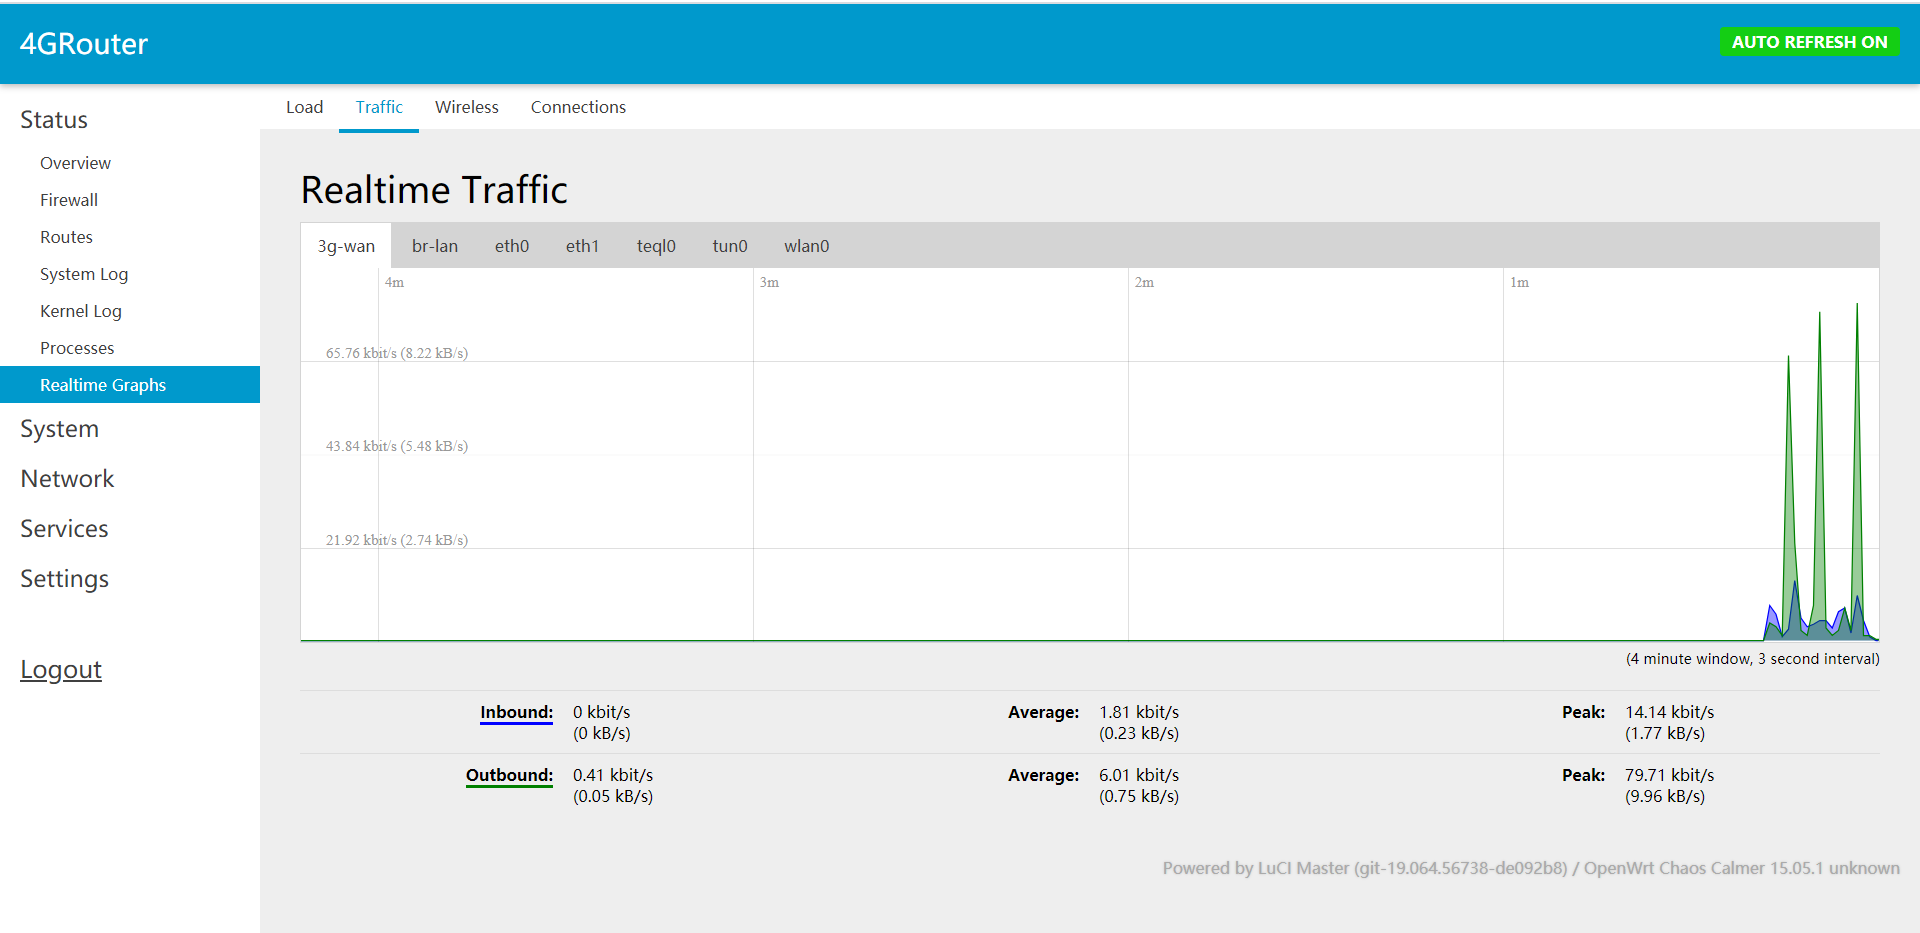
\includegraphics[totalheight=\tempheight]{immagini/interfacciar4g_traffic}
		\caption{Grafico del traffico}
	\end{subfigure}

	\medskip

	\begin{subfigure}[b]{\textwidth}
		\centering%
		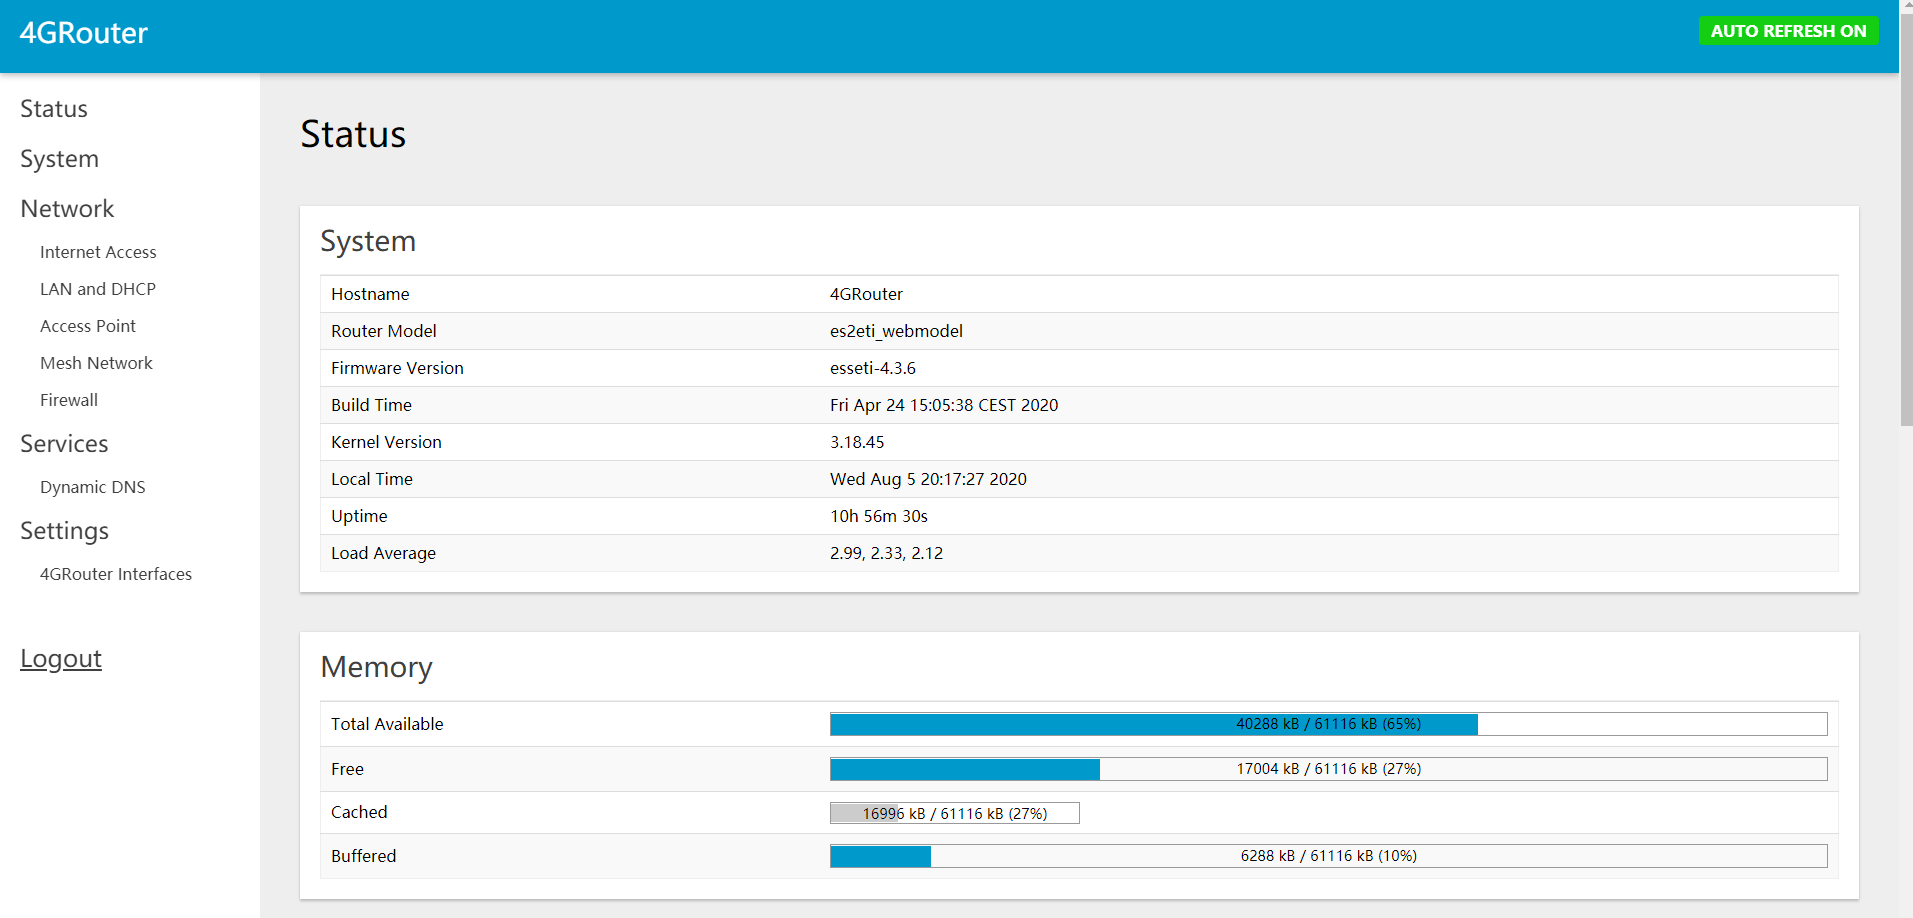
\includegraphics[totalheight=1.8\tempheight]{immagini/interfacciar4g_status}
		\caption{Schermata con stato riassuntivo}
	\end{subfigure}
	\caption{Interfaccia web Esse-ti 4G.Router}

\end{figure}

Per semplicità si farà riferimento all'\textit{Esse-ti 4G.Router} chiamandolo semplicemente \textit{Router}.

\subsection{VPS OVHCloud}

La VPS ha il solo vincolo di dover avere un'ip pubblico e una connessione a internet abbastanza veloce. Dovrà infatti sopportare un traffico simmetrico in upload / download.

Per la realizzazione della topologia è stata selezionata una macchina VPS del provider \textit{OVHCloud}, con le seguenti caratteristiche:

\begin{itemize}
	\item 2 core virtuali
	\item 4Gb di memoria ram
	\item 80Gb di storage NVMe
	\item 500Mbps simmetrici di banda
	\item ipv4 pubblico
	\item Ubuntu 16.04
\end{itemize}

Per semplicità si farà riferimento alla \textit{VPS OVHCloud} come \textit{Server}.

\subsection{Host domotico}

Per simulare un'host domotico ed effettuare le varie operazioni di testing è stata usata una \textit{raspberry pi}, con le utility \textit{ping} e \textit{tracepath}.

\subsection{Macchina del cliente \workinprogress}

Per avere la massima flessibilità la macchina del cliente deve essere generica e non deve necessitare di nessuna configurazione specifica. Data la scelta di usare OpenVPN come provider VPN, e dato che OpenVPN è cross-platform, la macchina del cliente non ha specifiche di sistema operativo. L'unica necessità è di avere il client OpenVPN installato sul sistema, ad esempio:

\todo[don't like forse lo tolgo]

\begin{itemize}
	\item con sistema operativo Windows si deve scaricare l'eseguibile dal \href{https://openvpn.net/client-connect-vpn-for-windows/}{sito ufficiale}
	\item su linux è sufficiente cercare nei repository ufficiali della distribuzione che si sta usando, es. Ubuntu: \code{apt-get install openvpn}.
\end{itemize}


